\documentclass[12pt]{article}
\usepackage[utf8]{inputenc}
\usepackage{graphicx}
\usepackage{amsmath}
\usepackage{hyperref}
\usepackage{amsfonts}
\usepackage{amssymb}
\usepackage{graphicx}
\usepackage{subcaption}
\usepackage{float}
\usepackage{tikz}
\usepackage{listings}
\usepackage{color}
\usepackage{parskip}
\usepackage{hyperref}
\hypersetup{
    colorlinks=true,
    linkcolor=black,
    citecolor=black,
    filecolor=black,
    urlcolor=black
}
\usepackage[left=1in,right=1in,top=1in,bottom=1in]{geometry}

\title{Rotacrypt: Rotational Mechanics as a Cryptographic Primitive}
\author{Teo Honda Scully}
\date{}

\begin{document}

\maketitle

\begin{abstract}
...TBD...
\end{abstract}

\tableofcontents

\newpage

\section{Introduction}
<...>

\subsection{Review of Rubik's Cubes}
Ah, the Rubik's Cube—the iconic toy that bedevils and delights in equal measure. Born from the ingenious mind of Ernő Rubik in 1974, it's more than just a puzzle. Forget mere child's play; this cube is chaos in the physical. Just kidding. To go from the state of chaos to order, one only needs to know a solving protocol of which many exist.

Max Park, the current world record holder (11 June 2023) for the 2-handed solve, obliterated the cube in a mind-blowing 3.13 seconds. Lucky scramble? Hardly. Yiheng Wang, who holds the world record average-of-five, clocks in at a dizzying 4.48 second mean solve time throughout the five solves.\footnote{An average-of-five is determined by taking the average of the three "middle" solves in a session of five scramble. In other words, the worst and best solve time are dropped from the calculation for the average.} And no, I won't depress you by mentioning his tender age of nine years old. But let's not divert. The Rubik's Cube--a mathematical marvel and a cipher waiting to be cracked. \\

\begin{figure}[h]
    \centering
    \begin{minipage}[c]{0.2\textwidth}
        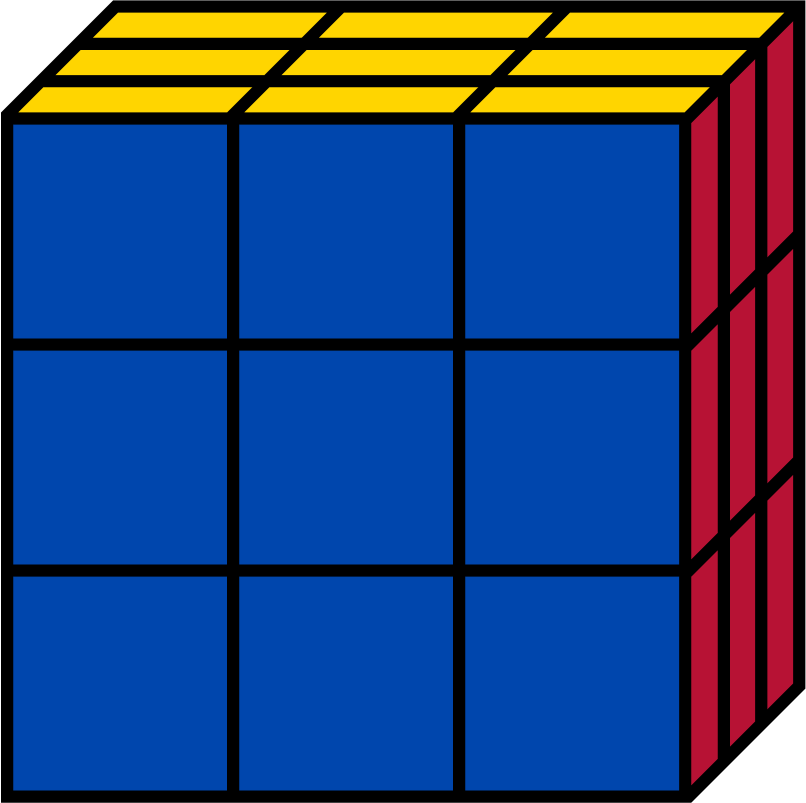
\includegraphics[scale=0.1]{cube.png}
    \end{minipage}
    \begin{minipage}[c]{0.2\textwidth}
        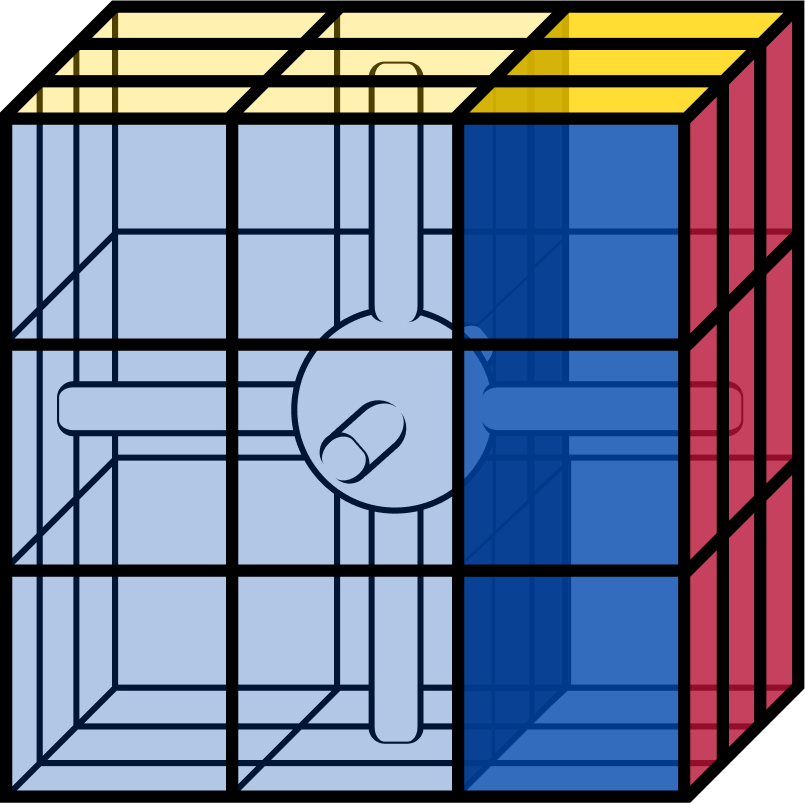
\includegraphics[scale=0.1]{core_r_highlight.png}
    \end{minipage}
    \begin{minipage}[c]{0.05\textwidth}
        \centering
        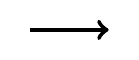
\begin{tikzpicture}
            \draw [->, ultra thick] (0,0.5)--(1,0.5);
        \end{tikzpicture}
    \end{minipage}
    \hspace{0.5cm}
    \begin{minipage}[c]{0.2\textwidth}
        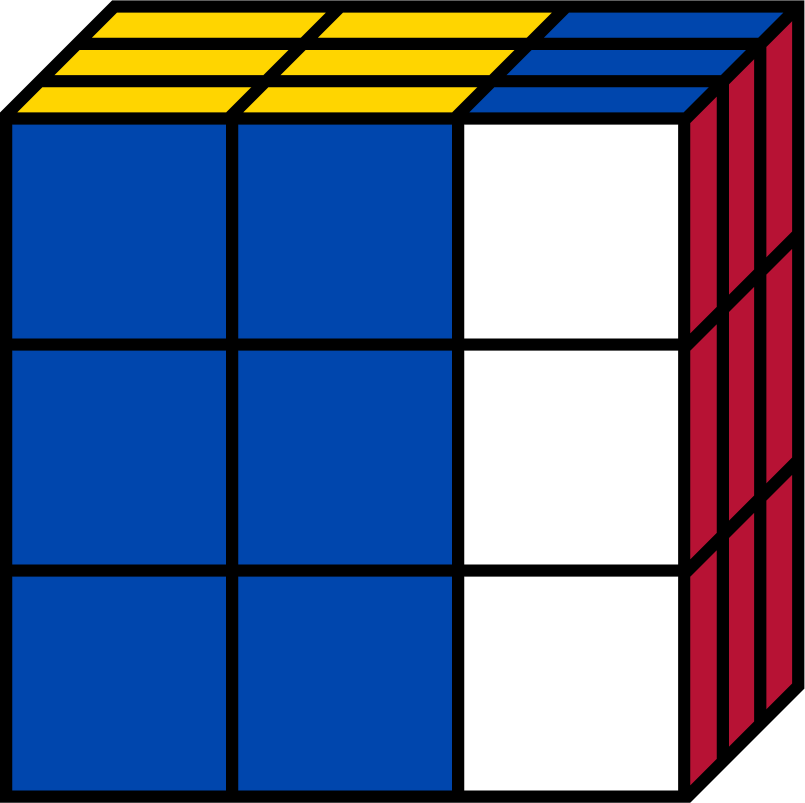
\includegraphics[scale=0.1]{cube_r.png}
    \end{minipage}
    \begin{minipage}[c]{0.2\textwidth}
        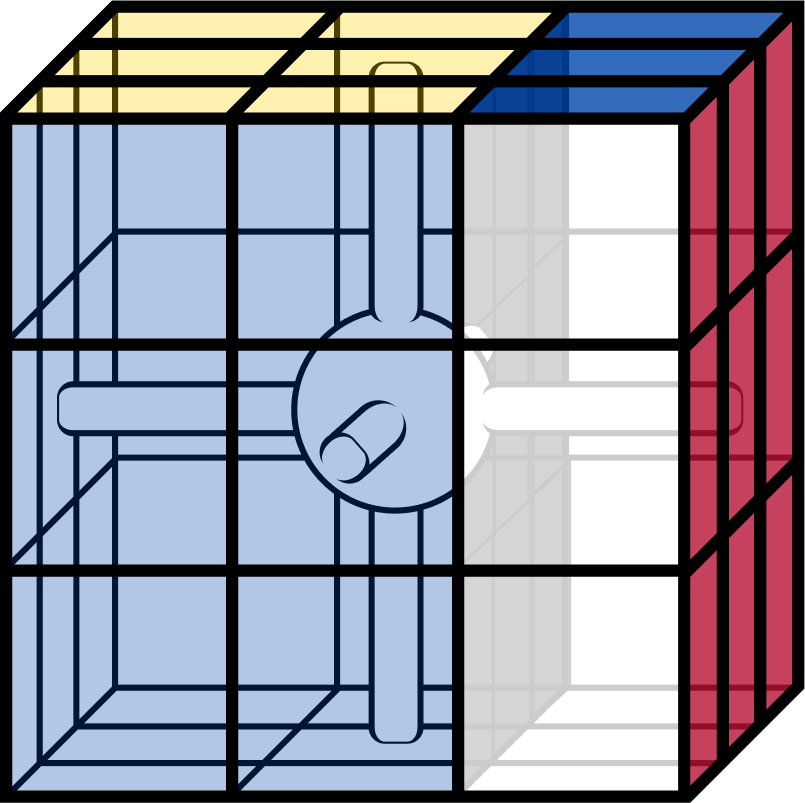
\includegraphics[scale=0.1]{core_r_transform.png}
    \end{minipage}
    \caption{A visualization of the \textit{R} operation (rotating the right layer clockwise).}
\end{figure}

Let's dive into the mechanics of the 3x3x3 puzzle. The cube boasts centers, edges, and corners. These single-colored center pieces serve as the invariant axis around which the peripheral cubies rotate. The six unit colors are yellow, blue, red, green, orange, and white.

\begin{figure}[h]
    \hfill 
    \begin{minipage}[c]{0.2\textwidth} 
        \centering
        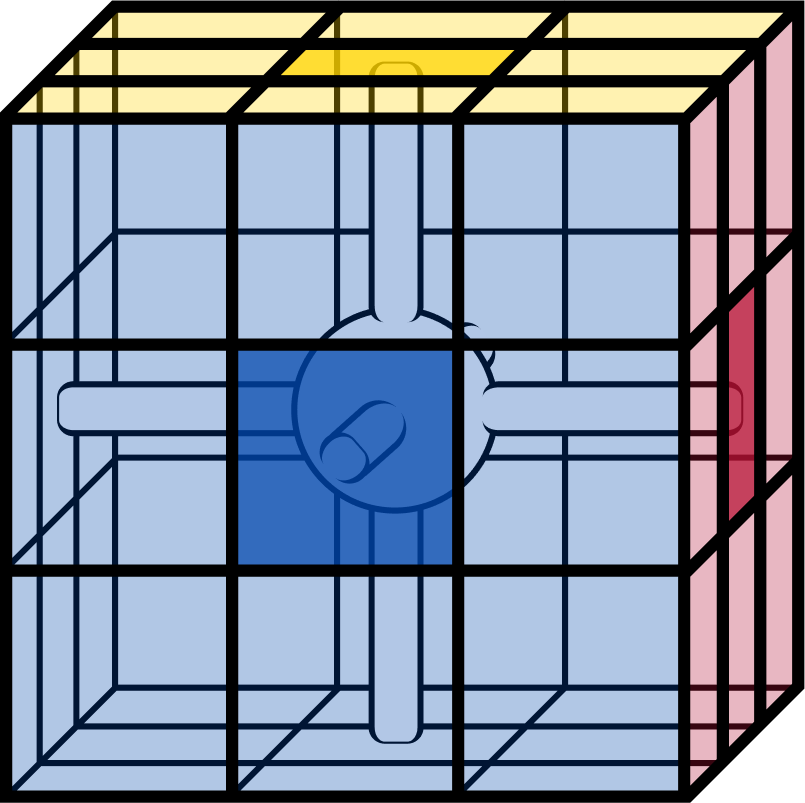
\includegraphics[scale=0.1]{core.png}
    \end{minipage}
    \hfill 
    \begin{minipage}[c]{0.59\textwidth} 
        \vspace*{\fill} 
        A visualization of a 3x3x3 cube. The cube has 6 faces, each with 9 stickers. Notably, this means that there exists 54 different unit tiles on the cube. The cube has 43,252,003,274,489,856,000 possible states.\footnotemark
        \vspace*{\fill}
    \end{minipage}
    \hfill 
\end{figure}
\footnotetext{This number is calculated by considering the \( 8 \) corners, each with \( 3 \) orientations, and the \( 12 \) edges, each with \( 2 \) orientations.}

For instance, if the cube is held with a yellow top and blue front, the red and orange faces will invariably be to the right and left, respectively. In fact, the red and orange center pieces will \textit{always} be opposites, as will the blue-green and white-yellow pairs of center pieces.\\

\begin{figure}[h]
    \centering
    \begin{minipage}[c]{0.2\textwidth}
        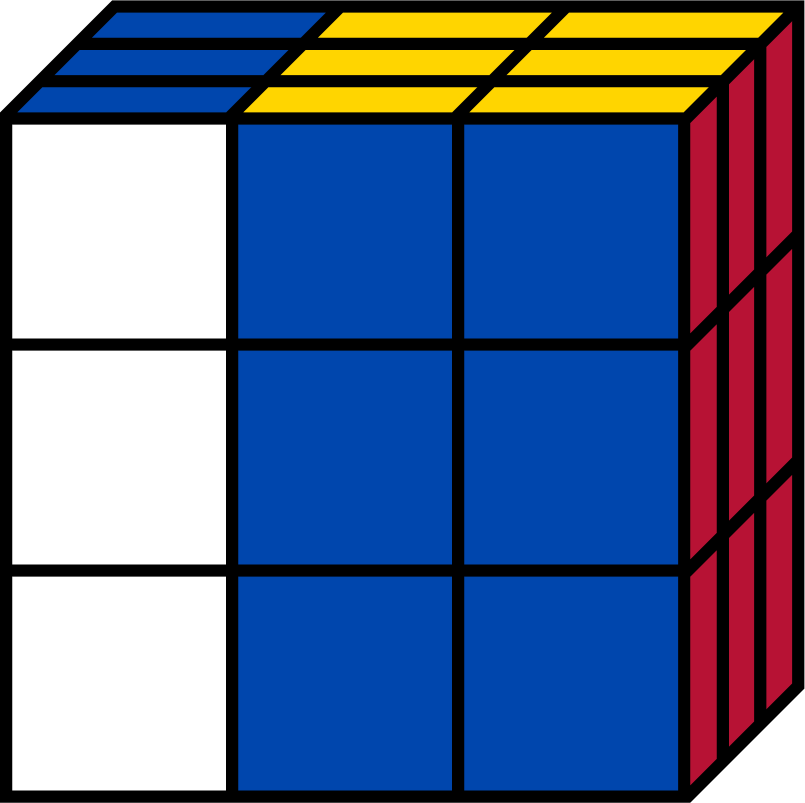
\includegraphics[scale=0.1]{cubeLp.png}
    \end{minipage}
    \begin{minipage}[c]{0.05\textwidth}
        \centering
        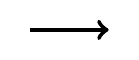
\begin{tikzpicture}
            \draw [->, ultra thick] (0,0.5)--(1,0.5);
        \end{tikzpicture}
    \end{minipage}
    \hspace{0.5cm}
    \begin{minipage}[c]{0.2\textwidth}
        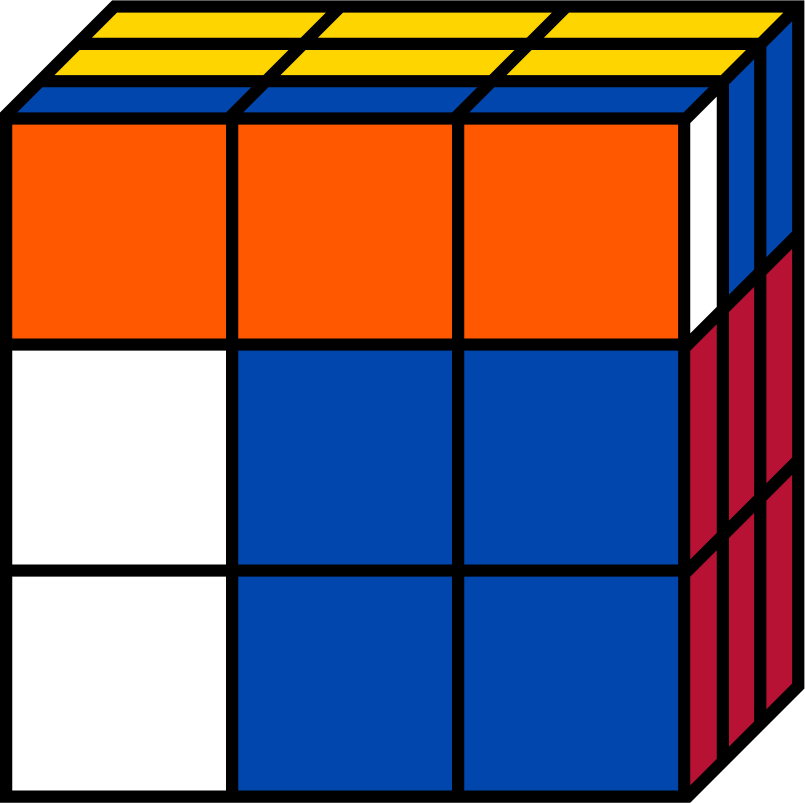
\includegraphics[scale=0.1]{cubeLpUp.png}
    \end{minipage}
    \begin{minipage}[c]{0.05\textwidth}
        \centering
        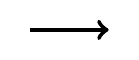
\begin{tikzpicture}
            \draw [->, ultra thick] (0,0.5)--(1,0.5);
        \end{tikzpicture}
    \end{minipage}
    \hspace{0.5cm}
    \begin{minipage}[c]{0.2\textwidth}
        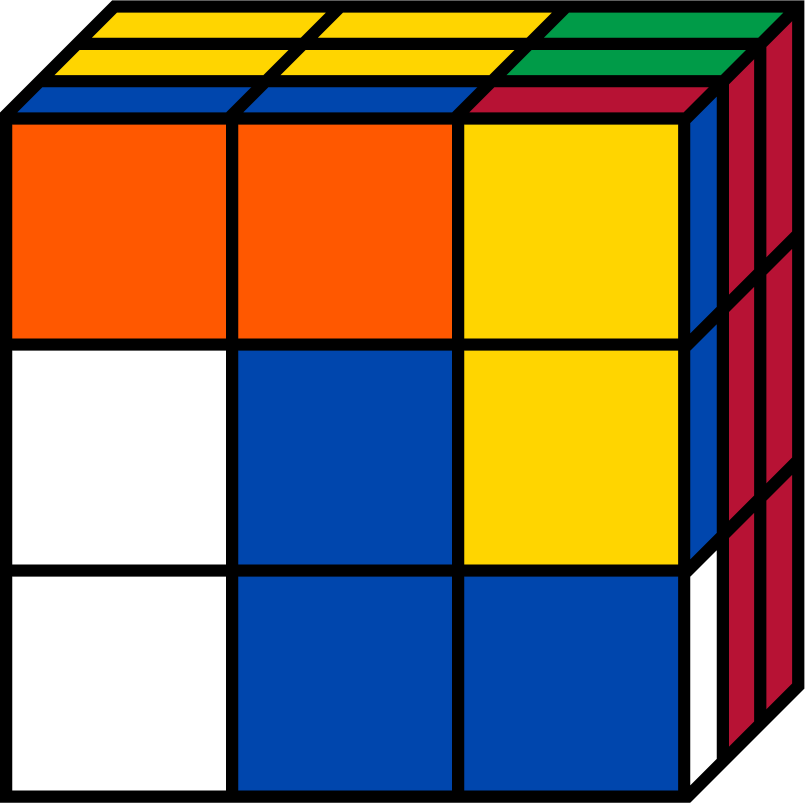
\includegraphics[scale=0.1]{cubeLpUpRp.png}
    \end{minipage}
    \caption{A visualization of the \textit{L' U' R'} operation(s).}
\end{figure}

\subsection{Notation for Cube Operations}

The notation used to describe the movements and algorithms for solving the Rubik's Cube is standardized to facilitate easy understanding and sharing of solutions. Each face of the cube is designated by an uppercase letter:

\begin{itemize}
    \item \textbf{U} - Up (Top Layer)
    \item \textbf{D} - Down (Bottom Layer)
    \item \textbf{L} - Left (Left Layer)
    \item \textbf{R} - Right (Right Layer)
    \item \textbf{F} - Front (Front Layer)
    \item \textbf{B} - Back (Back Layer)
\end{itemize}

The following symbols are appended to these letters to indicate the direction of rotation:

\begin{itemize}
    \item No symbol - 90-degree clockwise rotation
    \item \textbf{'} (apostrophe) - 90-degree counterclockwise rotation
    \item \textbf{2} - 180-degree rotation (either direction)
\end{itemize}

For example, the sequence \textit{L' U' R'} would indicate a counterclockwise rotation of the left layer, followed by a counterclockwise rotation of the top layer, and finally, a counterclockwise rotation of the right layer.

\subsection{God's Number}
In the realm of 3x3x3 Rubik's Cubes, \textit{God's Number} is a term used to denote the maximum number of moves required to solve any scrambled cube. It has been proven that any cube can be solved in 20 moves or fewer (the citation can be found in the \textit{References} section). This concept is an intriguing insight into the mathematical efficiency of the cube's design.

Furthermore, this means that any scramble can be reached with 20 moves or fewer. This is a key point to keep in mind when considering the security of the cube as a cryptographic primitive as well as for key size considerations.\\

\subsection{Combinatorial Explosion with Multiple Cubes}
Let us consider the number of possible states for a single 3x3x3 Rubik's Cube, which is \(43,252,003,274,489,856,000\). When chaining together the combinations of two different cubes, the number of combined states is \((43,252,003,274,489,856,000)^2\).

This squaring occurs because each state of the first cube can pair with every state of the second cube, yielding \(43,252,003,274,489,856,000 \times 43,252,003,274,489,856,000\). Mathematically, the set of possible states becomes the Cartesian product of the two sets of states, leading to an exponential increase in complexity.

One intriguing aspect of chaining multiple Rubik's Cubes is the exponential growth in the state space. Let \( N \) represent the number of unique states for a single Rubik's Cube. For \( k \) chained Rubik's Cubes, the total number of unique states becomes \( N^k \). This exponential increase serves a critical function: it substantially minimizes the likelihood of collisions whilst simultaneously increasing the difficulty of brute-force attacks.

\section{Overview}

\subsection{Scheme Overview}

\begin{figure}[h]
    \centering
    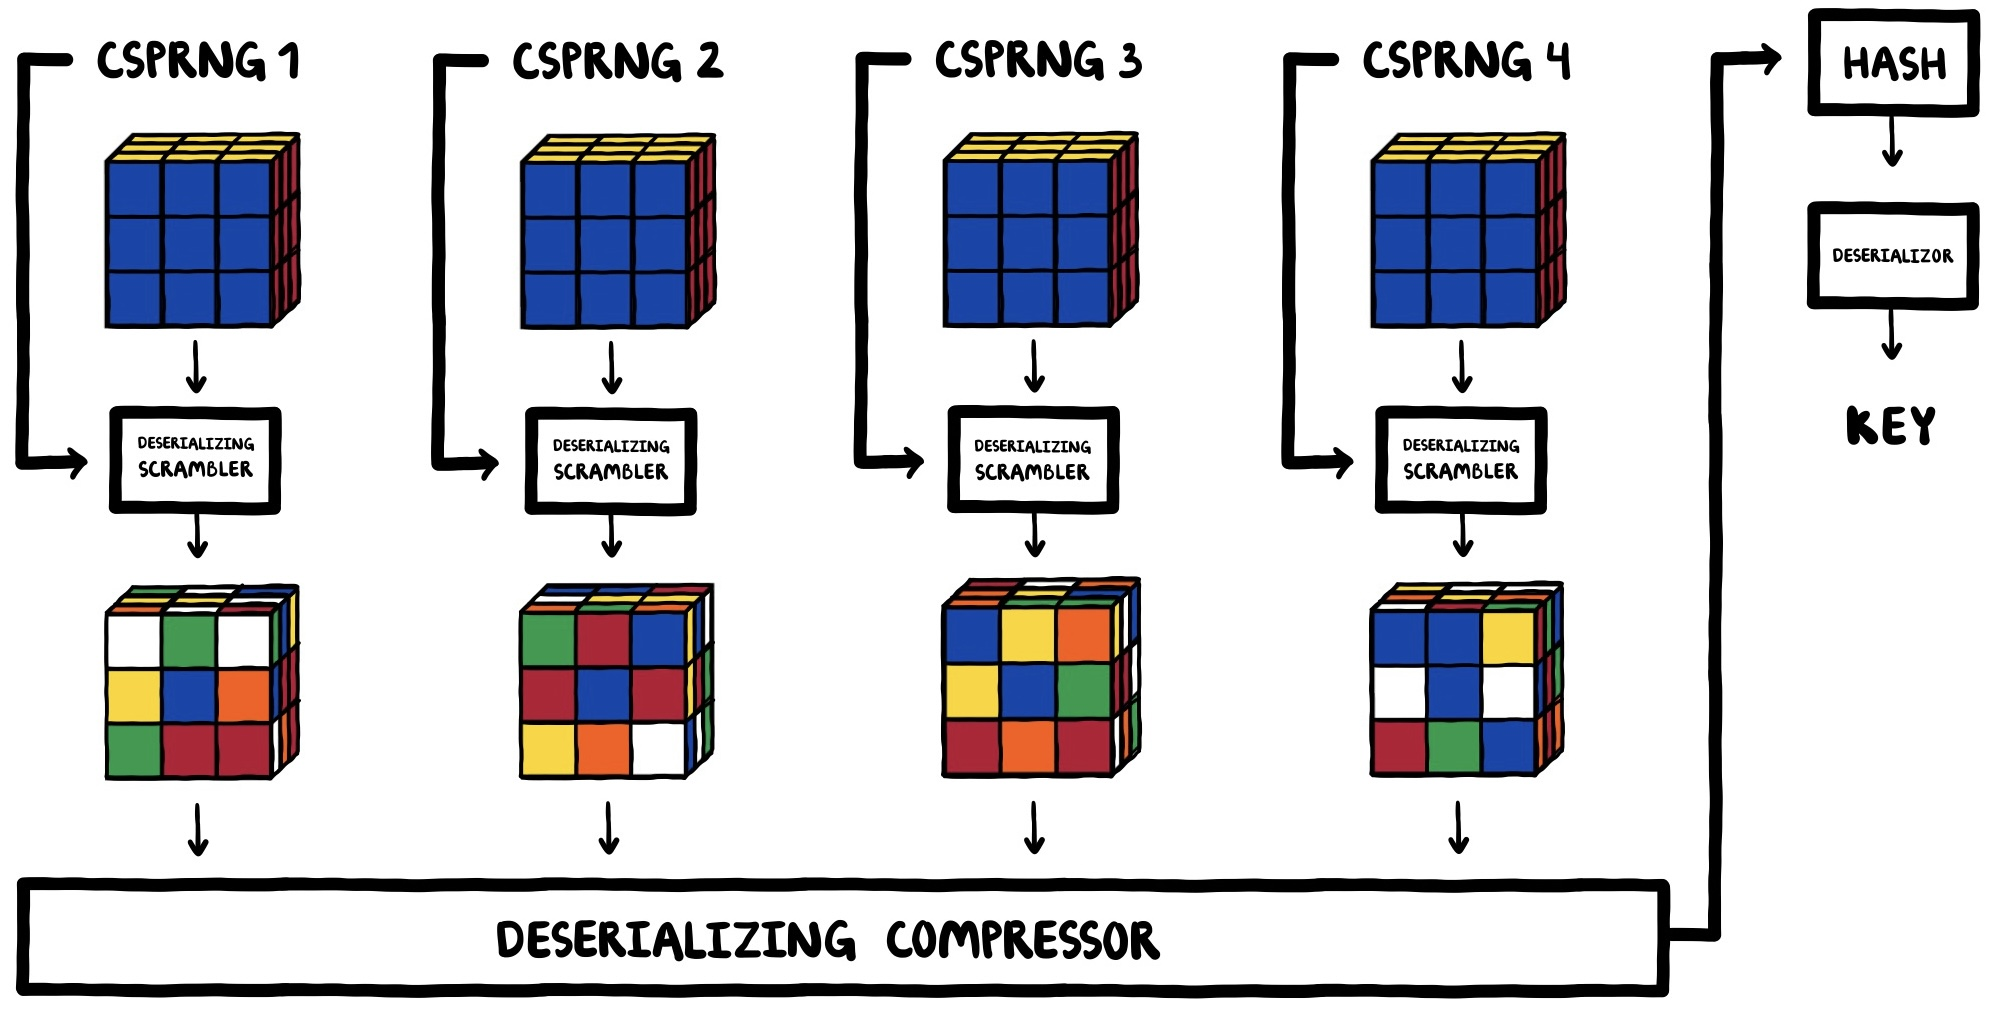
\includegraphics[width=\textwidth]{keygen.jpg}
    \caption{beep boop}
\end{figure}

\subsection{Purpose}
There is no purpose. I was told to not make a cryptosystem, so I did the opposite.

\subsection{Intended Usage}
<...>

\section{3x3x3 Implementation}
<...>

\subsection{Data Structure Breakdown}
<...>

\subsection{Augmented SPEFFZ Mapping}
<...>

\subsection{Cyclic Transformations}

\section{Key Generation}
<...>

\subsection{4-Cube Initialization}
<...>

\subsection{Master-Key Serialization}
<...>

\subsection{Sub-Key Generation}
<...>

\section{Encryption}
<...>

\subsection{Plaintext Setup With S-Box Transformations On Chunks}
<...>

\subsection{Cube Mapping Procedure}
<...>

\subsection{Encryption Algorithm}
<...>

\section{Decryption}
<...>

\end{document}
